\documentclass[11pt,letterpaper]{article}
\usepackage[lmargin=1in,rmargin=1in,tmargin=1in,bmargin=1in]{geometry}
\usepackage{../style/homework}
\usepackage{../style/commands}
\setbool{quotetype}{false} % True: Side; False: Under
\setbool{hideans}{false} % Student: True; Instructor: False

% -------------------
% Content
% -------------------
\begin{document}

\homework{20: Due 11/30}{The philosophy of the school room in one generation will be the philosophy of government in the next.}{Abraham Lincoln}

% Problem 1
\problem{10} For each of the following quadratic functions, i.e. functions which can be written as $f(x)= ax^2 + bx + c$, identify $a, b, c$:
	\begin{enumerate}[(a)]
	\item $2x^2 - 5x + 7$
	\item $6x + 9 - x^2$
	\item $x^2 - 16$
	\item $(x + 1)^2$
	\item $(x - 2)(x + 3)$
	\end{enumerate} \pspace

\sol 
\begin{enumerate}[(a)]
\item We have $a= 2$, $b= -5$, and $c= 7$. \pspace

\item Because $6x + 9 - x^2= -x^2 + 6x + 9$, we have $a= -1$, $b= 6$, and $c= 9$. \pspace

\item Because $x^2 - 16= x^2 + 0x - 16$, we have $a= 1$, $b= 0$, and $c= -16$. \pspace

\item Because $(x + 1)^2= (x + 1)(x + 1)= x^2 + x + x + 1= x^2 + 2x + 1$, we have $a= 1$, $b= 2$, and $c= 1$. \pspace

\item Becase $(x - 2)(x + 3)= x^2 + 3x - 2x - 6= x^2 + x - 6$, we have $a= 1$, $b= 1$, and $c= -6$. 
\end{enumerate}



\newpage



% Problem 2
\problem{10} Consider the quadratic function $f(x)= 4 - (x - 2)^2$.
	\begin{enumerate}[(a)]
	\item Determine if the given parabola opens upwards or downwards.
	\item Is the parabola convex or concave?
	\item Does the function $f(x)$ have a maximum or a minimum?
	\item Find the vertex and axis of symmetry. 
	\item Find the maximum or minimum value of $f(x)$. 
	\item Sketch a graph of $f(x)$ on the plot below. 
	\end{enumerate} \pspace

\sol 
\begin{enumerate}[(a)]
\item Observe $f(x)= 4 - (x - 2)^2= -(x - 2)^2 + 4$ is in the form $a(x - p)^2 + q$ with $a= -1$, $p= 2$, and $q= 4$. Because $a= -1 < 0$, the parabola opens downwards. 

\item Because the parabola opens downwards, we know that the parabola is concave. 

\item Because the parabola opens downwards, the function $f(x)$ has a maximum. 

\item If $f(x)$ has the form $a(x - p)^2 + q$, then $f(x)$ is a quadratic function with vertex $(p , q)$ and axis of symmetry $x= p$. Observe $f(x)= 4 - (x - 2)^2= -(x - 2)^2 + 4$ is in the form $a(x - p)^2 + q$ with $a= -1$, $p= 2$, and $q= 4$. Therefore, the vertex is $(2, 4)$ and the axis of symmetry is $x= 2$. 

\item Because $f(x)$ opens downwards, there is no minimum value for $f(x)$; however, there is a maximum value. The maximum value is the $y$-coordinate of the vertex. Because the vertex is $(2, 4)$, the maximum value for $f(x)$ is 4. 

\item If $f(x)$ has the form $a(x - p)^2 + q$, then $f(x)$ is a quadratic function with vertex $(p , q)$ and axis of symmetry $x= p$. Furthermore, if $a > 0$ then the parabola opens upwards and if $a < 0$ the parabola opens downwards. Observe $f(x)= 4 - (x - 2)^2= -(x - 2)^2 + 4$ is in the form $a(x - p)^2 + q$ with $a= -1$, $p= 2$, and $q= 4$. Therefore, the parabola opens downwards, the vertex is $(2, 4)$, and the axis of symmetry is $x= 2$. This gives the sketch below. \vfill
\end{enumerate}

	\[
	\fbox{
	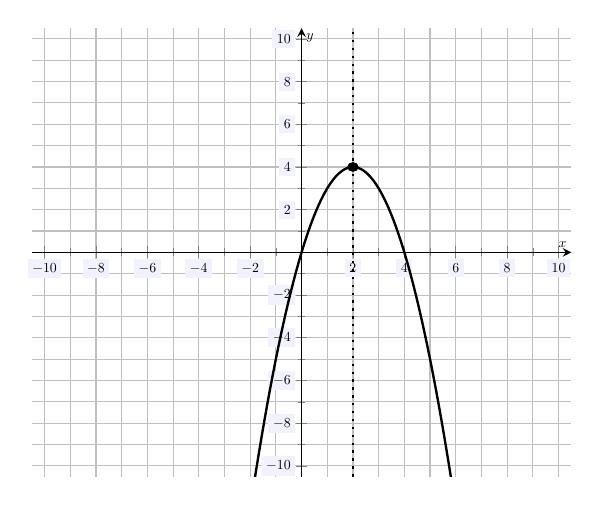
\begin{tikzpicture}[scale=1,every node/.style={scale=0.5}]
	\begin{axis}[
	grid=both,
	axis lines=middle,
	ticklabel style={fill=blue!5!white},
	xmin= -10.5, xmax=10.5,
	ymin= -10.5, ymax=10.5,
	xtick={-10,-8,-6,-4,-2,0,2,4,6,8,10},
	ytick={-10,-8,-6,-4,-2,0,2,4,6,8,10},
	minor tick = {-10,-9,...,10},
	xlabel=\(x\),ylabel=\(y\),
	]
	\draw[line width= 0.03cm, dotted] (2,-10.5) -- (2,10.5);
	\addplot[samples= 100, domain= -3:8, line width= 0.03cm] ({x}, {4 - (x - 2)^2});
	\draw[fill=black] (2, 4) circle (0.2);
	\end{axis}
	\end{tikzpicture}
	}
	\]



\newpage



% Problem 3
\problem{10} Showing all your work, put $f(x)= 2x^2 - 12x - 13$ into vertex form. Also, find the vertex and axis of symmetry for $f(x)$. \pspace

\sol If we complete the square, we have\dots
	\[
	\begin{aligned}
	f(x)&= 2x^2 - 12x - 13 \\
	&= 2 \left( x^2 - 6x - \dfrac{13}{2} \right) \\
	&= 2 \left( x^2 - 6x + 3^2 - 3^2 - \dfrac{13}{2} \right) \\
	&= 2 \left( (x^2 - 6x + 9) - 9 - \dfrac{13}{2} \right) \\
	&= 2 \left( (x - 3)^2 - \dfrac{18}{2} - \dfrac{13}{2} \right) \\
	&= 2 \left( (x - 3)^2 - \dfrac{31}{2} \right) \\
	&= 2(x - 3)^2 - 31
	\end{aligned}
	\]
The vertex form of $f(x)$ is then $f(x)= 2(x - 3)^2 - 31$. Therefore, the vertex is $(3, -31)$ and the axis of symmetry is $x= 3$. \pspace

If we use the `evaluation method', we know the vertex occurs at $x= - \frac{b}{2a}$. We find the $y$-coordinate by evaluation $f(x)$ at this value. Therefore, we have\dots
	\[
	\begin{aligned}
	x&= -\dfrac{b}{2a}= -\dfrac{-12}{2(2)}= -\dfrac{-12}{4}= -(-3)= 3 \\
	f(3)&= 2(3^2) - 12(3) - 13= 2(9) - 12(3) - 13= 18 - 36 - 13= -31
	\end{aligned}
	\]
Given a quadratic function with leading coefficient $a$ and vertex $(p, q)$, the function is $f(x)= a(x - p)^2 + q$. From the work above, we know that the vertex is $(3, -31)$. Because $f(x)= 2x^2 - 12x - 13$, we know that $a= 2$. Therefore, $f(x)= 2(x - 3)^2 - 31$ is the vertex form of $f(x)$. Again, from the work above, we know that the vertex is $(3, -31)$ and that the axis of symmetry is $x= 3$. 


\end{document}